\documentclass{article}
\usepackage[utf8]{inputenc}
\usepackage[margin=1in]{geometry}
\usepackage{hyperref}
\usepackage{listings}
\usepackage{longtable}
\usepackage{array}
\usepackage{float}
\usepackage{graphicx}
\usepackage{subcaption} % for subfigures
\graphicspath{{./assets}} % adjust to your path

\begin{document}
\title{Segmentation Engine Documentation}
\maketitle

\section{Scope}
This document describes the Segmentation Engine, a C++ HTTP service for route analysis and segment extraction. It has been prepared in accordance with ISO/IEC/IEEE 26514:2008, which defines structure and content for software user documentation.

\section{Normative References}
\begin{itemize}
\item ISO/IEC/IEEE 26514:2008 -- Systems and software engineering -- Requirements for designers and developers of user documentation.
\item ISO 8601:2019 -- Date and time representation.
\end{itemize}

\section{Terms and Definitions}
\begin{description}
\item[Segment] A contiguous portion of a route, represented as GeoJSON geometry and associated metadata.
\item[Route signal] A sampled representation of map variables (elevation, curvature, \ldots) indexed by distance along the route.
\item[Bounding box] Geographic region defined by west, south, east and north coordinates.
\end{description}

\section{System Overview}
The engine exposes a RESTful API that receives map data, builds route signals, performs wavelet based segmentation and persists results to a MySQL database. The major modules are:
\begin{itemize}
\item \textbf{core}: algorithmic components such as the route signal builder, segmentation logic and wavelet utilities.
\item \textbf{http}: request routing and REST endpoint handlers built on \texttt{cpp-httplib}.
\item \textbf{infra}: database adapter for MySQL persistence.
\item \textbf{models}: C++ types representing OSRM responses, segments and configuration parameters.
\end{itemize}

\section{Installation and Operation}
\subsection{Prerequisites}
CMake~3.15 or newer, a C++17 capable compiler, Docker and a running MySQL server.

\subsection{Build and Deployment}
The provided script builds and runs the engine inside a Docker container:
\begin{verbatim}
./build_and_deploy.sh
\end{verbatim}
It performs three steps:
\begin{enumerate}
  \item Build an image tagged \texttt{segmentation\_engine:latest}.
  \item Remove any existing container named \texttt{segmentation\_container}.
  \item Launch a new container on port~5005 with MySQL parameters (\texttt{DB\_HOST}, \texttt{DB\_PORT}, \texttt{DB\_USER}, \texttt{DB\_PASS}, \texttt{DB\_NAME}) supplied via the environment.
\end{enumerate}

Internally, the script issues the following Docker commands:
\begin{verbatim}
docker build -t segmentation_engine:latest .
docker rm -f segmentation_container >/dev/null 2>&1 || true
docker run -d --name segmentation_container --network host \
  -e DB_HOST=127.0.0.1 -e DB_PORT=3306 -e DB_USER=routeseg_user \
  -e DB_PASS=changeme-user -e DB_NAME=routeseg -p 5005:5005 \
  segmentation_engine:latest
\end{verbatim}
Container logs can be monitored via:\newline
\texttt{docker logs -f segmentation\_container}

For a manual build without Docker:
\begin{verbatim}
cmake -S . -B build
cmake --build build
./build/segmentation_engine
\end{verbatim}

\subsection{Configuration}
Runtime settings, including the HTTP port and enabled endpoints, are stored in \texttt{config/settings.json}. Database credentials are compiled into \texttt{src/main.cpp} and should be configured prior to deployment.

\subsection{Execution}
After deployment the service is reachable on \texttt{http://localhost:5005} and mounts the \texttt{public} directory under \texttt{/static}. POST and GET routes are registered from the configuration file.

To consolidate endpoints and avoid Cross-Origin Resource Sharing (CORS) issues, the parent
\texttt{segmentation} directory provides a lightweight Nginx proxy. From that directory run:
\begin{verbatim}
./proxy.sh
\end{verbatim}
The script starts a container named \texttt{quick-proxy} that forwards port~8081 to the
Segmentation Engine at \texttt{5005}, exposing the service at \texttt{http://localhost:8081}.
Additional proxy ports~8082 and~8083 target the viewer and database UI, allowing browser
clients to interact with all components through a single origin.

\section{REST API}
Table~\ref{tab:api} lists the available endpoints. JSON bodies use UTF-8 encoding and timestamps follow ISO~8601.
\begin{longtable}{>{\bfseries}p{5cm}p{9cm}}
\caption{REST endpoints}\label{tab:api}\\
Method/Path & Description \\\hline
\endfirsthead
Method/Path & Description \\\hline
\endhead
POST /upload & Accepts a map JSON file and stores it under \texttt{uploads/}. Returns the storage path.\\
GET /view?map=\emph{path} & Renders an interactive HTML viewer comparing raw OSRM geometry to the derived route signal.\\
GET /viewLab?map=\emph{path} & Redirects to the Signal Lab user interface.\\
GET /lab/meta?map=\emph{path} & Lists available uploads and optionally returns metadata for a specific map.\\
POST /lab/resample & Builds a route signal and resamples requested variables onto a uniform distance grid.\\
POST /wavelet & Performs wavelet-based terrain segmentation and optionally persists segments to the database.\\
GET /segments & Retrieves previously persisted segments intersecting a geographic bounding box.\\
\end{longtable}

\section{Algorithms}
Segmentation is accomplished by constructing a uniformly sampled route signal from the uploaded map and applying a wavelet-based energy detector. High energy regions correspond to changes in elevation or curvature and are converted into segments. Utilities in \texttt{core/wavelets} implement the FFT based rolling energy calculation. Existing segments can be matched against new routes to avoid redundant processing.

\section{Data Management}
Segment metadata is stored in a MySQL schema defined by \texttt{schema.sql}. The \texttt{infra::MySQLSegmentDB} component manages connections, inserts new segments and queries by bounding box.

\section{Error Handling and Logging}
Fatal signals (segmentation faults, aborts, arithmetic errors) are trapped and a stack trace is printed to the server log. Endpoint handlers translate exceptions into HTTP~500 responses containing a diagnostic message.

\section{Conformance}
The Segmentation Engine and this document use ISO~8601 timestamps and the terminology defined in ISO/IEC/IEEE~26514:2008. All numeric values are expressed using SI units.
\newpage
\section{Application Screenshots}

% === Dashboard & Data Upload ===
\subsection{Dashboard and Data Upload}
% [Context added]
 In line with ISO/IEC/IEEE 26514:2008 guidance on task-oriented documentation, this sequence demonstrates the primary user workflow: initial dashboard state, file transfer progression, confirmation of successful ingestion, and verification via route–OSRM alignment. The figure substantiates that the ingest–validate loop is operational end to end.

\label{sec:dashboard-upload}
\begin{figure}[H]
  \centering
  \begin{subfigure}[b]{0.48\textwidth}
    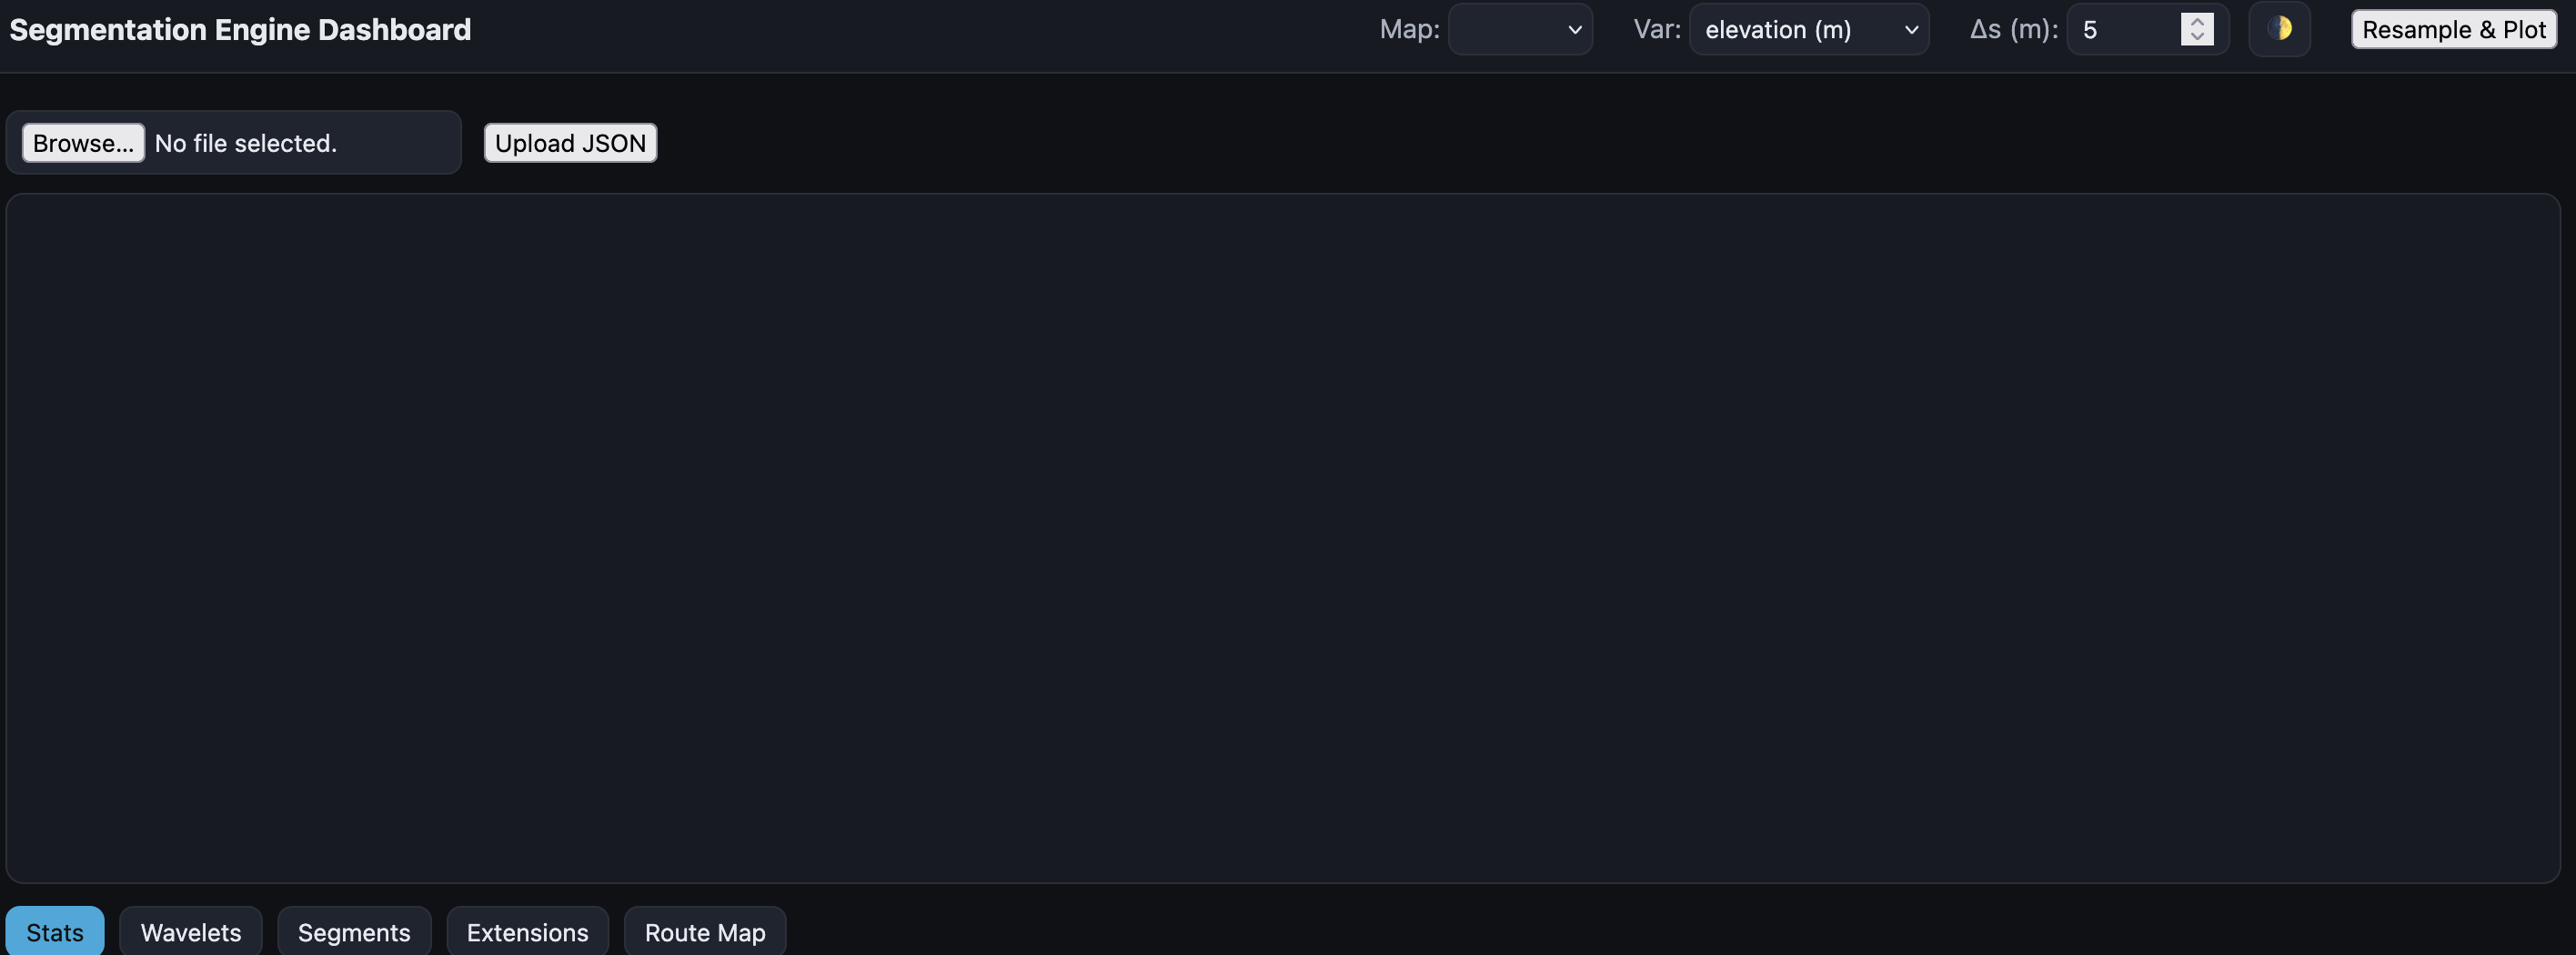
\includegraphics[width=\linewidth]{full_dashboard_default.png}
    \caption{Default dashboard on initial load.}
    \label{fig:dashboard-default}
  \end{subfigure}\hfill
  \begin{subfigure}[b]{0.48\textwidth}
    
\includegraphics[width=\linewidth]{upload_in_progress.png}
    \caption{Upload in progress.}
    \label{fig:upload-in-progress}
  \end{subfigure}

  \vspace{0.75em}
  \begin{subfigure}[b]{0.48\textwidth}
    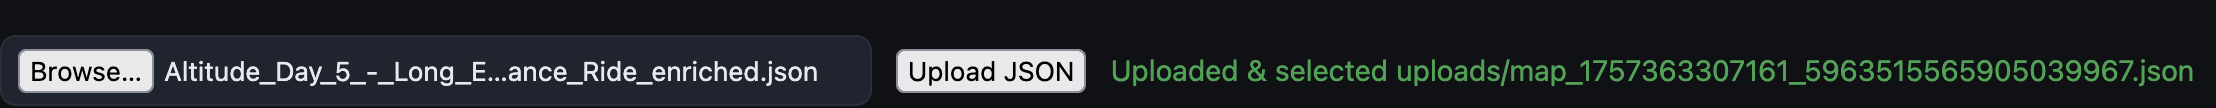
\includegraphics[width=\linewidth]{upload_complete.png}
    \caption{Upload complete.}
    \label{fig:upload-complete}
  \end{subfigure}\hfill
  \begin{subfigure}[b]{0.48\textwidth}
    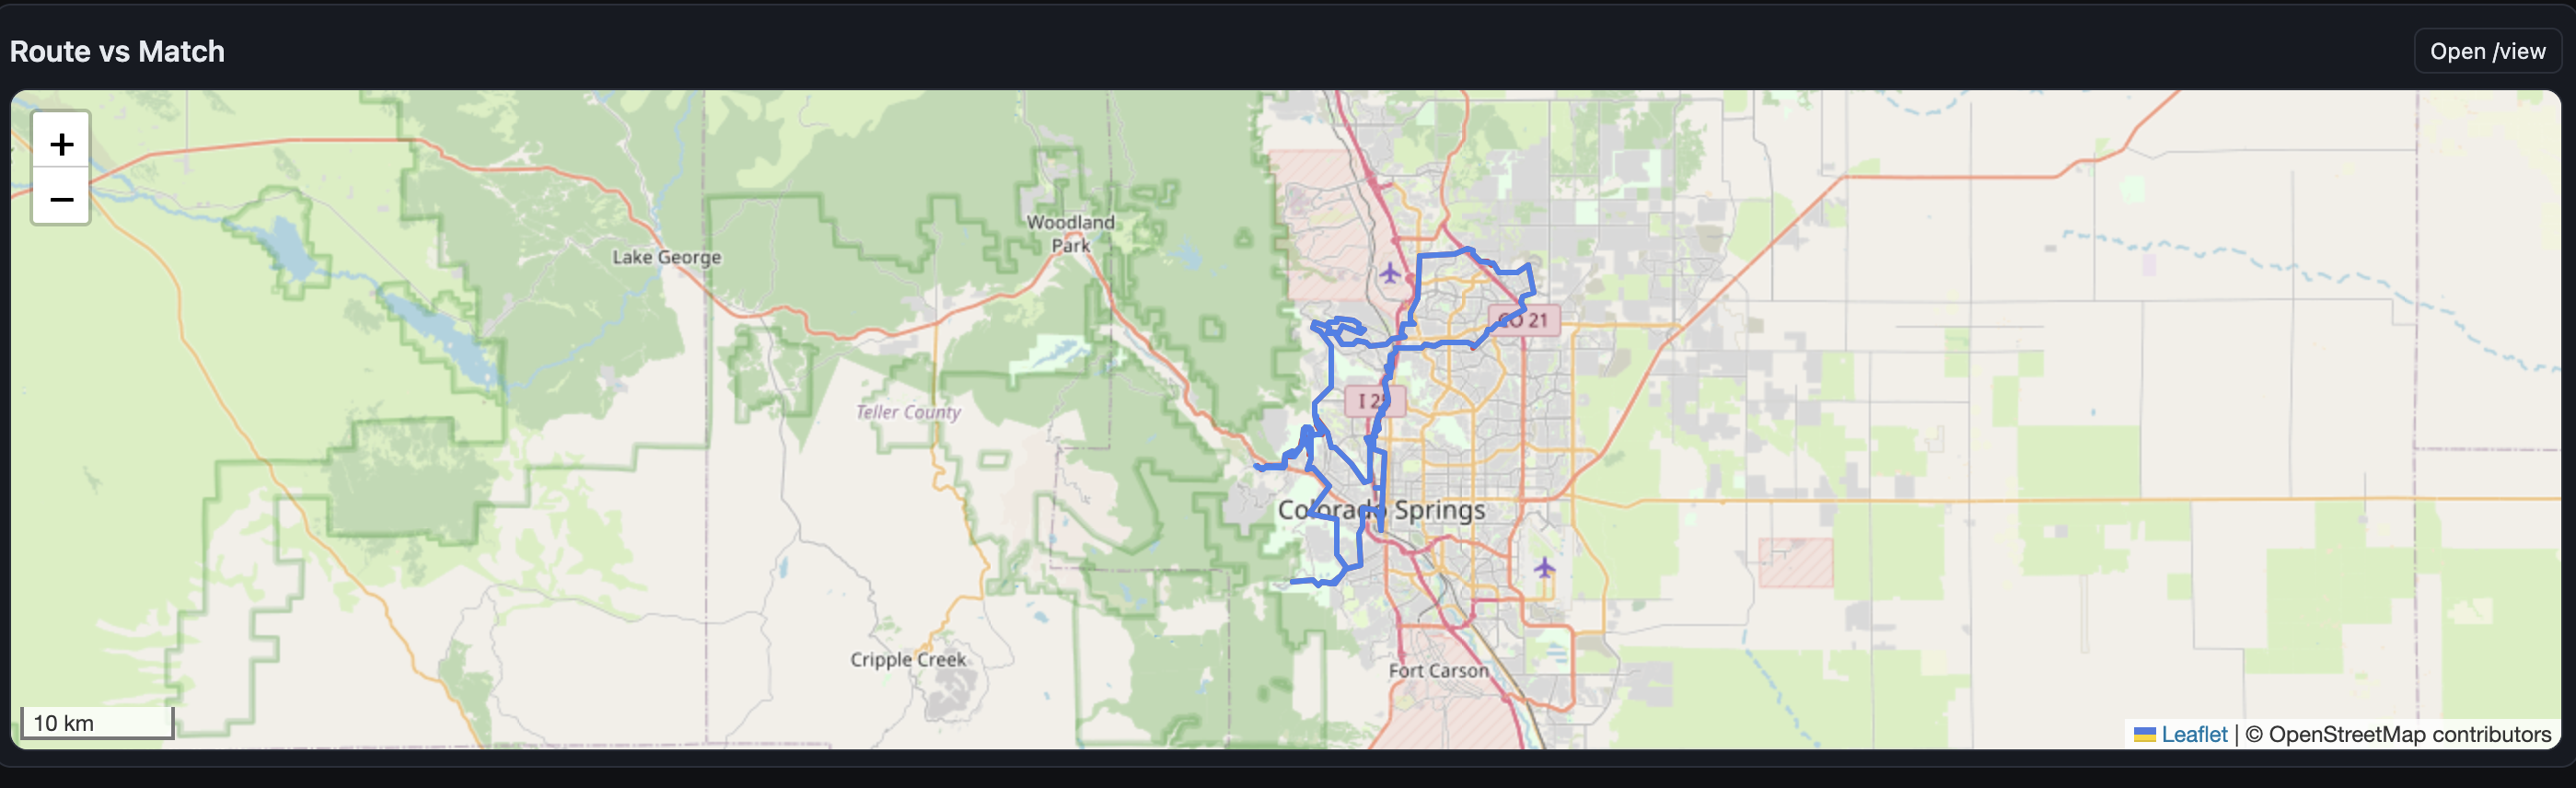
\includegraphics[width=\linewidth]{route_vs_match.png}
    \caption{Route vs matched geometry.}
    \label{fig:route-vs-match}
  \end{subfigure}

  \caption{Loading, uploading, and path matching workflow.}
  \label{fig:dashboard-upload}
\end{figure}

% === Database Viewer ===
\subsection{Database Viewer}
% [Context added]
 This view evidences persistence and retrieval capabilities as required by the standard's “data management and storage” descriptions. It shows that extracted segments are indexed, queryable, and auditable, supporting reproducibility of results and post hoc analysis.

\label{sec:db-viewer}
\begin{figure}[H]
  \centering
  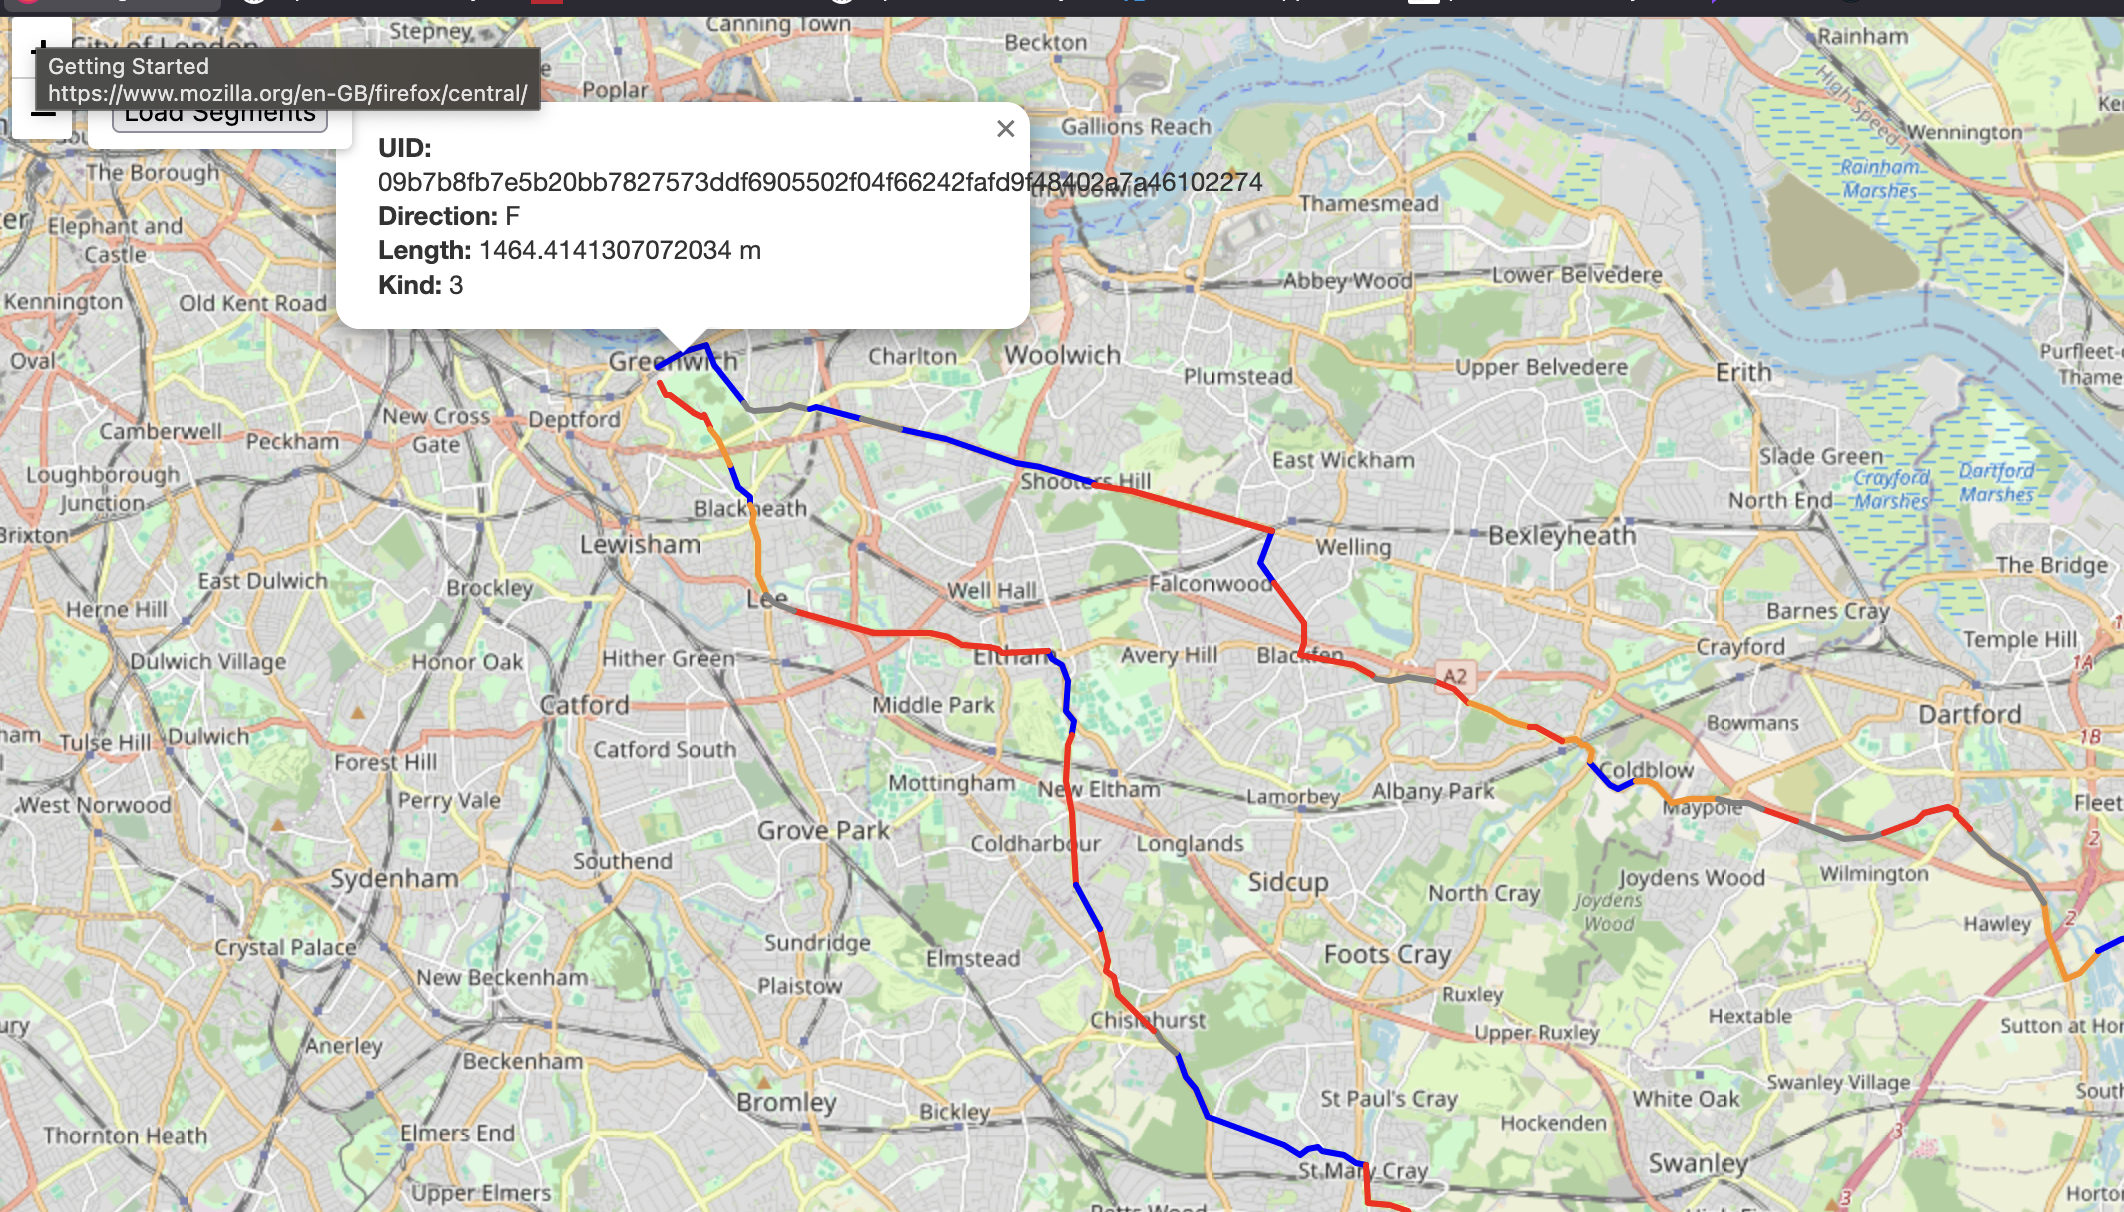
\includegraphics[width=0.7\linewidth]{segment_database_viewer.png}
  \caption{Interactive segment database inspector.}
  \label{fig:db-viewer}
\end{figure}

% === Signal & Wavelets ===
\subsection{Signal and Wavelet Panels}
% [Context added]
 These panels expose algorithm configuration and outputs, satisfying the standard’s expectation for clarity of computational steps. Elevation-versus-distance, tunable wavelet parameters, and the scalogram together justify threshold and segmentation choices, enabling readers to trace input settings to resultant segments.

\label{sec:signal-wavelet}
\begin{figure}[H]
  \centering
  \begin{subfigure}[b]{0.40\textwidth}
    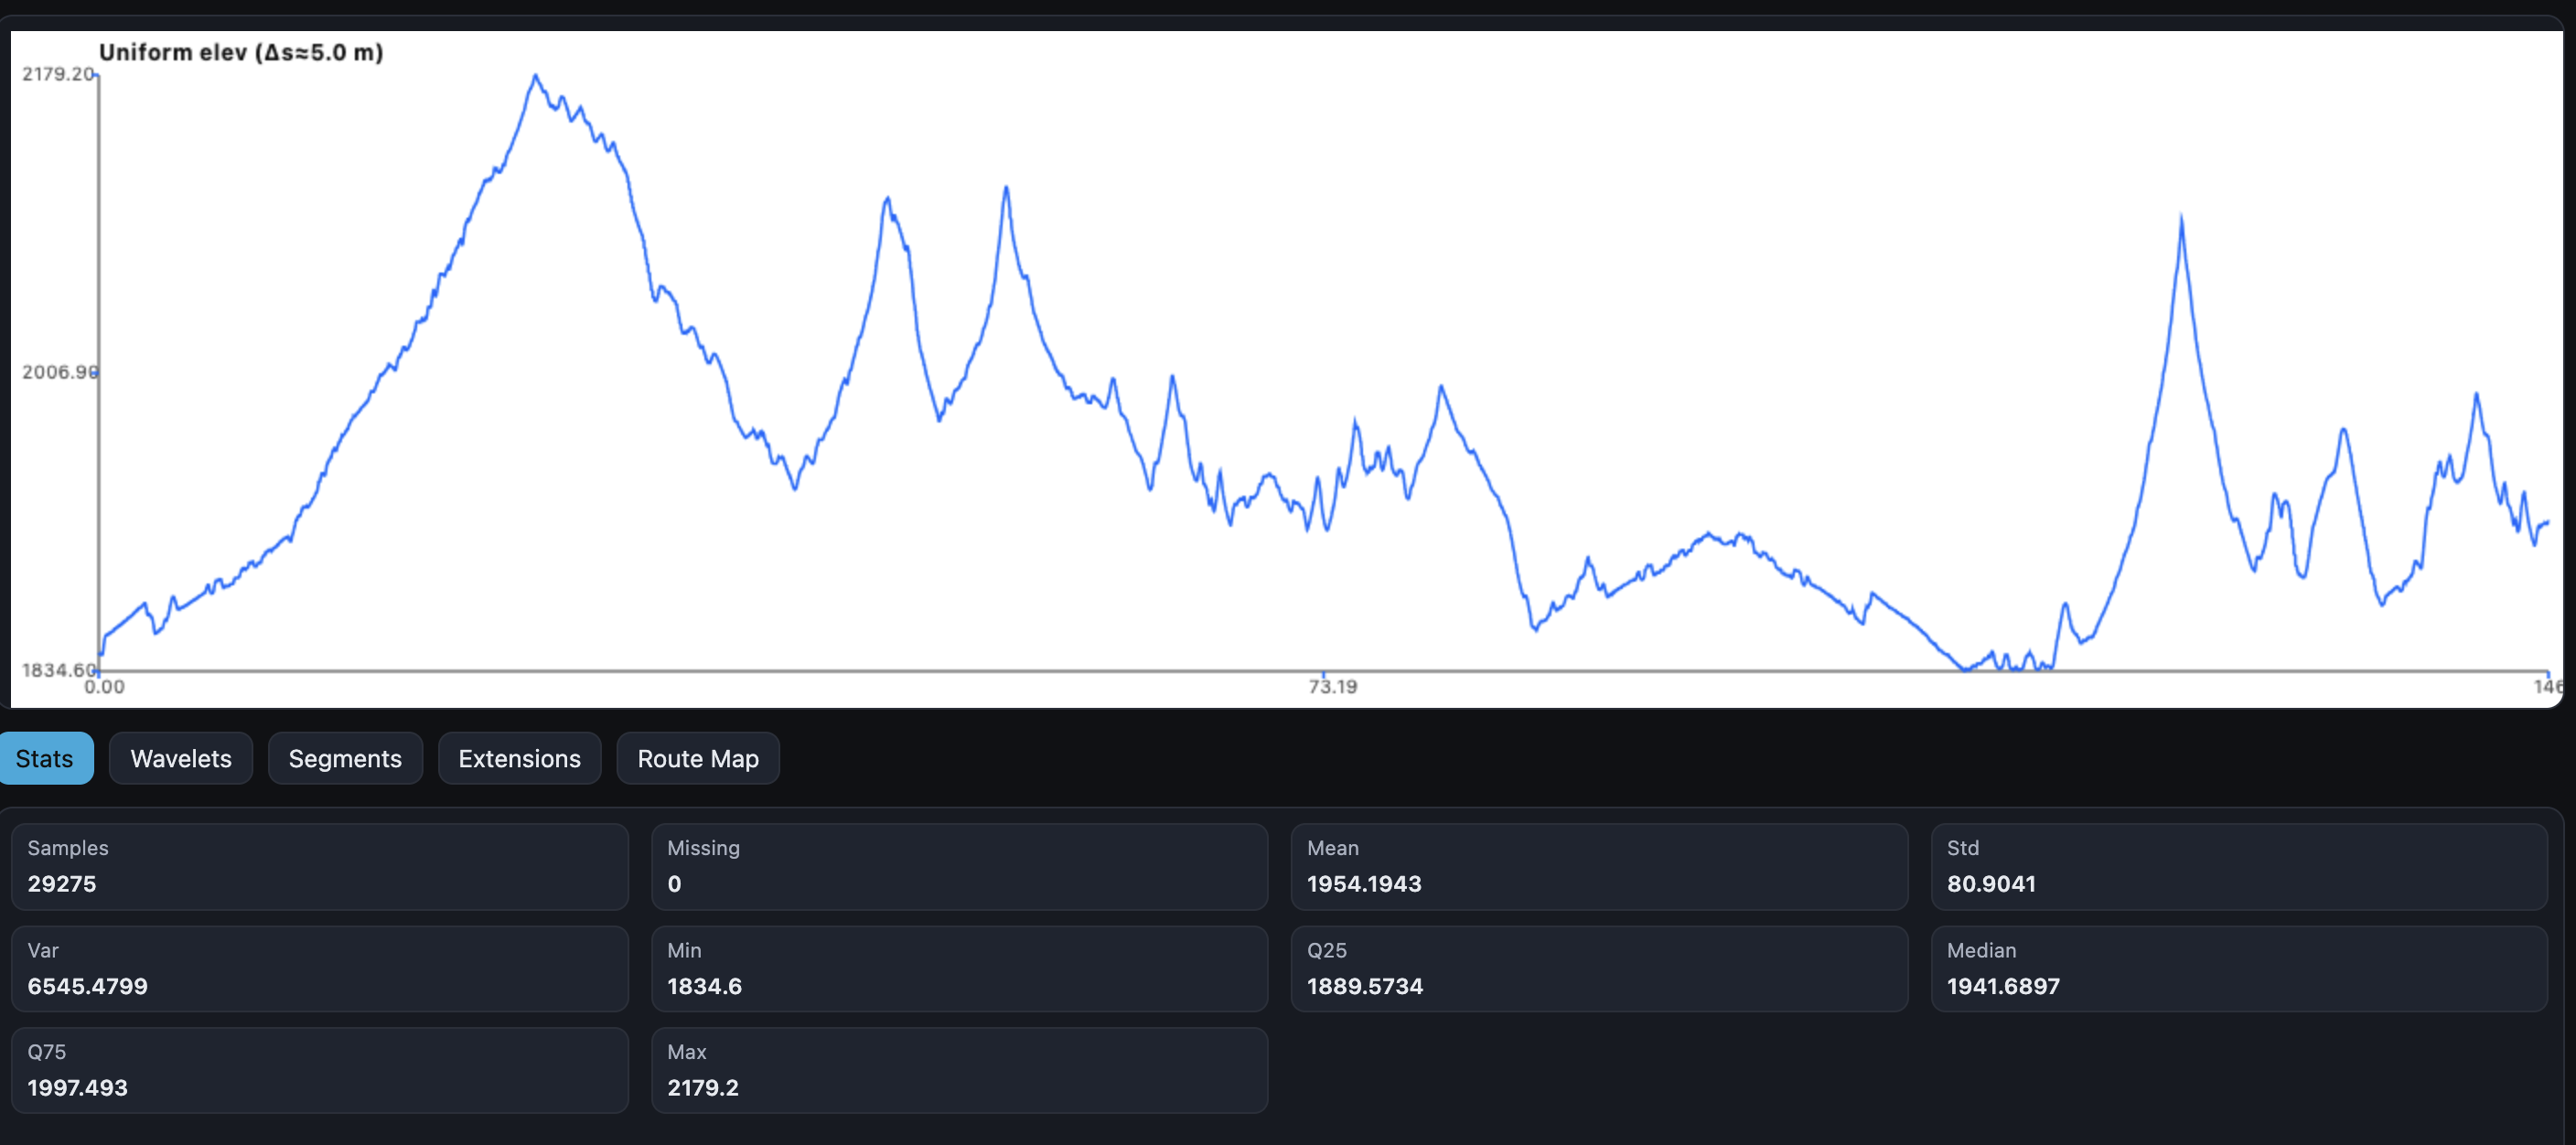
\includegraphics[width=\linewidth]{signals_elevation.png}
    \caption{Elevation view ($\Delta s = 5$m).}
    \label{fig:signal-elevation}
  \end{subfigure}\hfill
  \begin{subfigure}[b]{0.40\textwidth}
    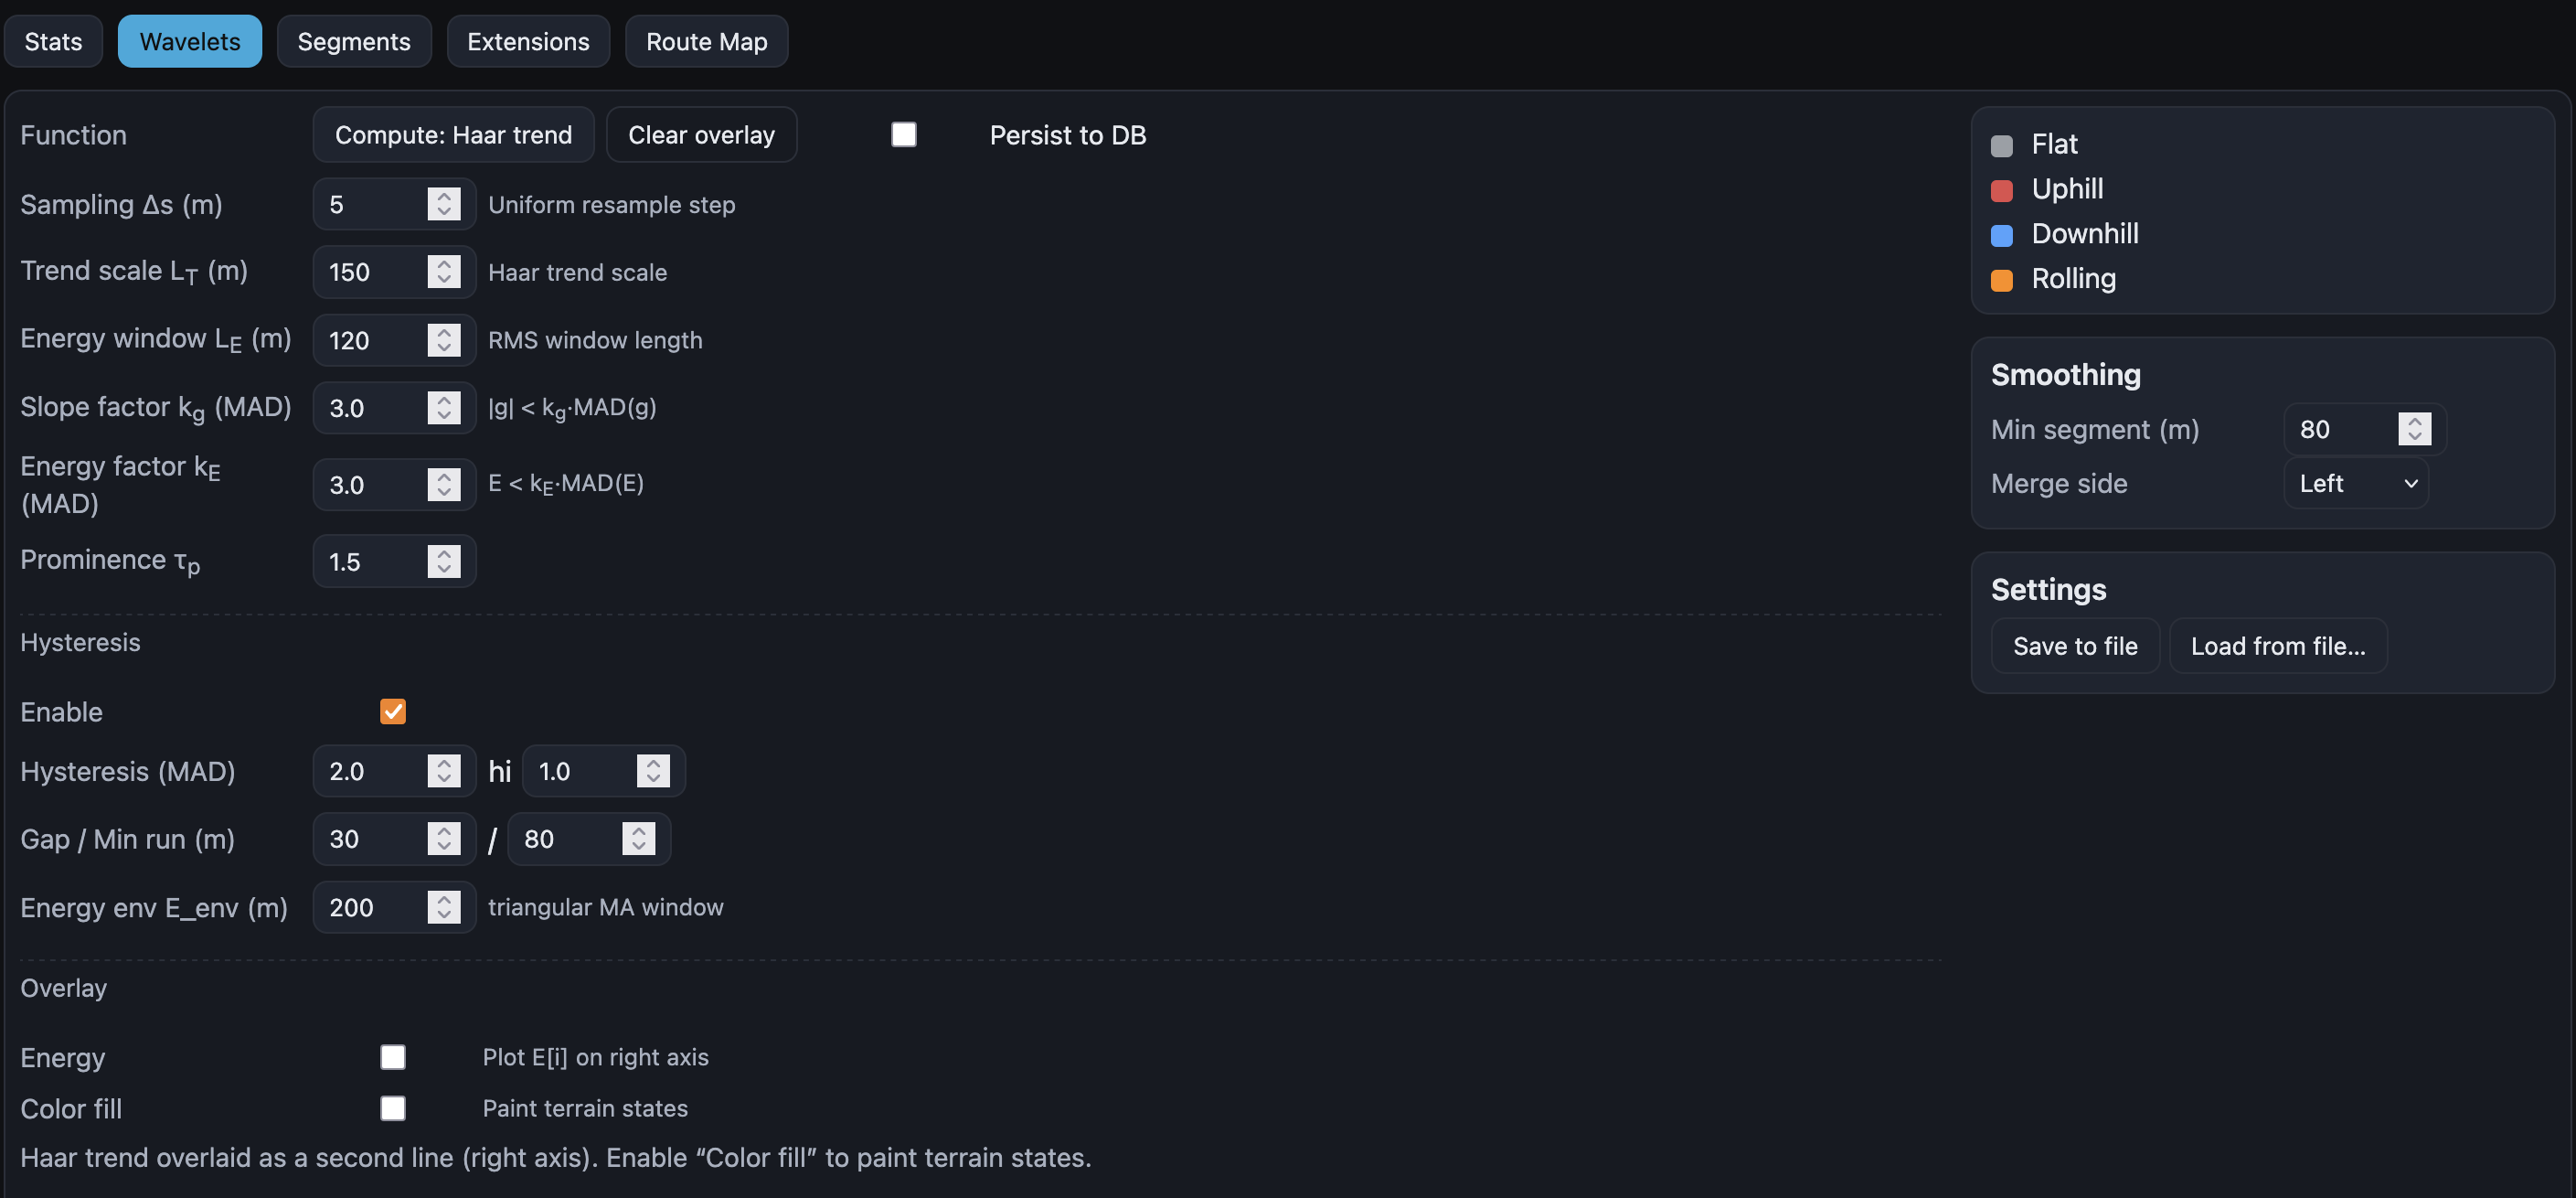
\includegraphics[width=\linewidth]{wavelet_controls.png}
    \caption{Wavelet controls.}
    \label{fig:wavelet-controls}
  \end{subfigure}

  \vspace{0.75em}
  \begin{subfigure}[b]{0.40\textwidth}
    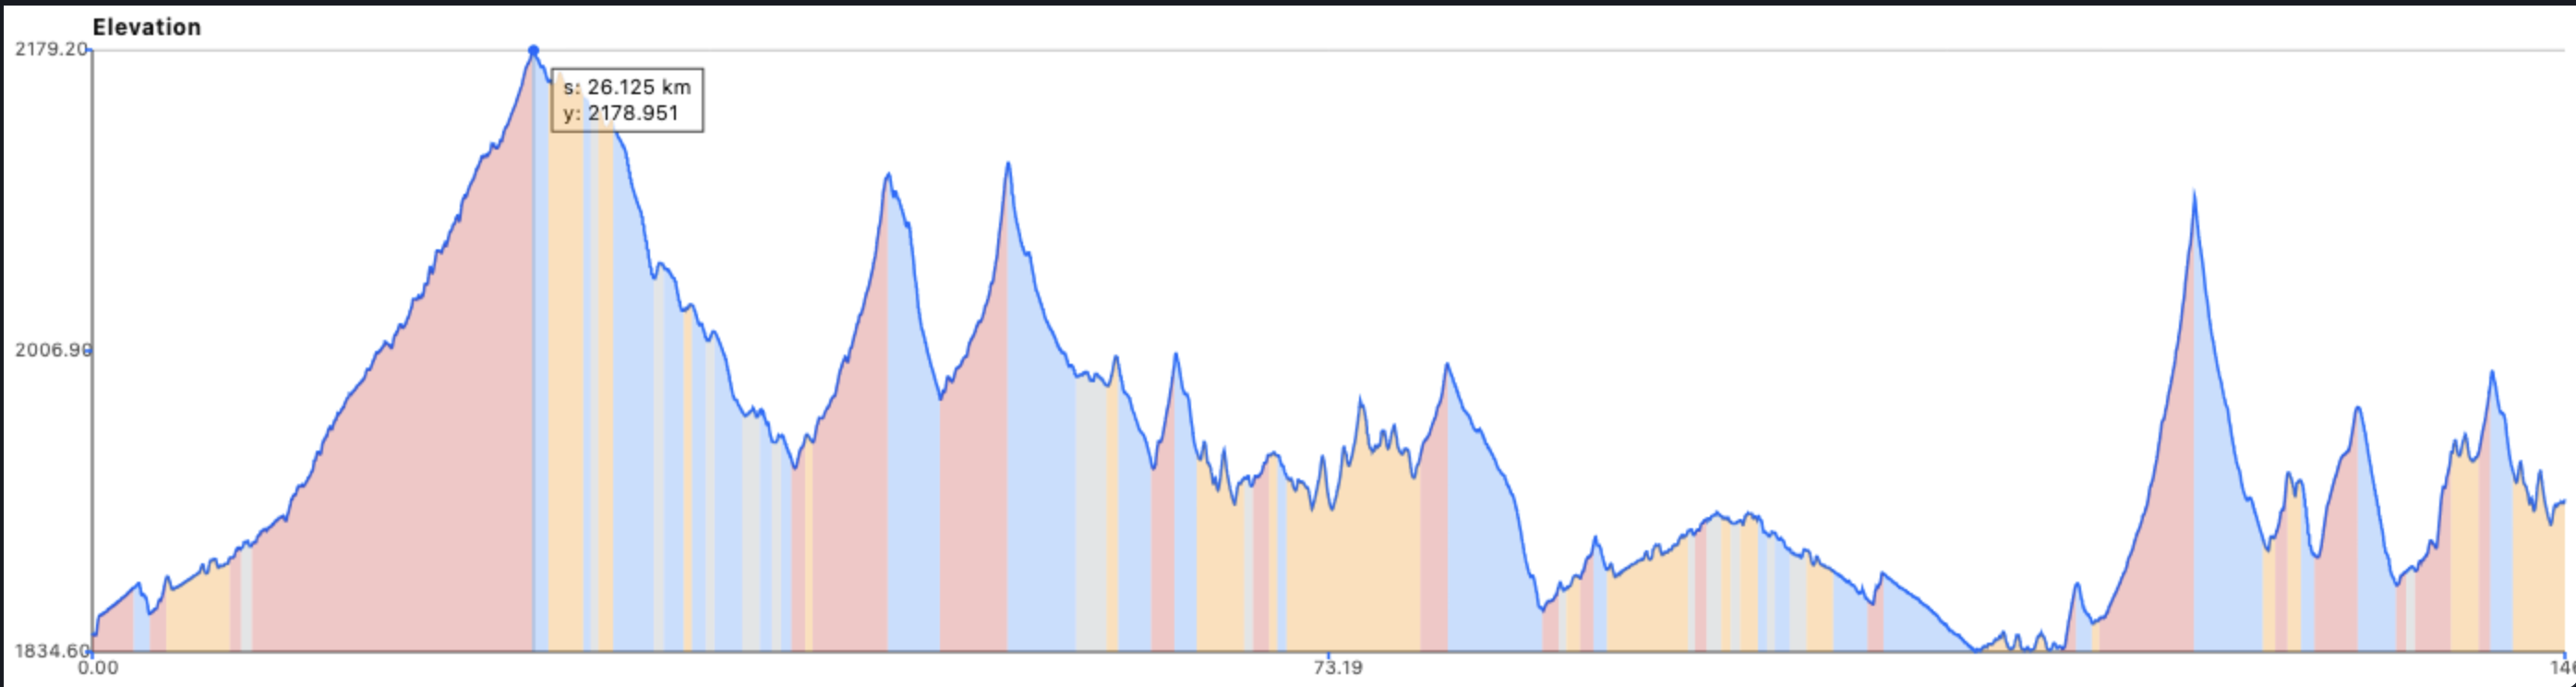
\includegraphics[width=\linewidth]{wavelet_display.png}
    \caption{Scalogram with trend overlay.}
    \label{fig:wavelet-display}
  \end{subfigure}\hfill
  \begin{subfigure}[b]{0.40\textwidth}
    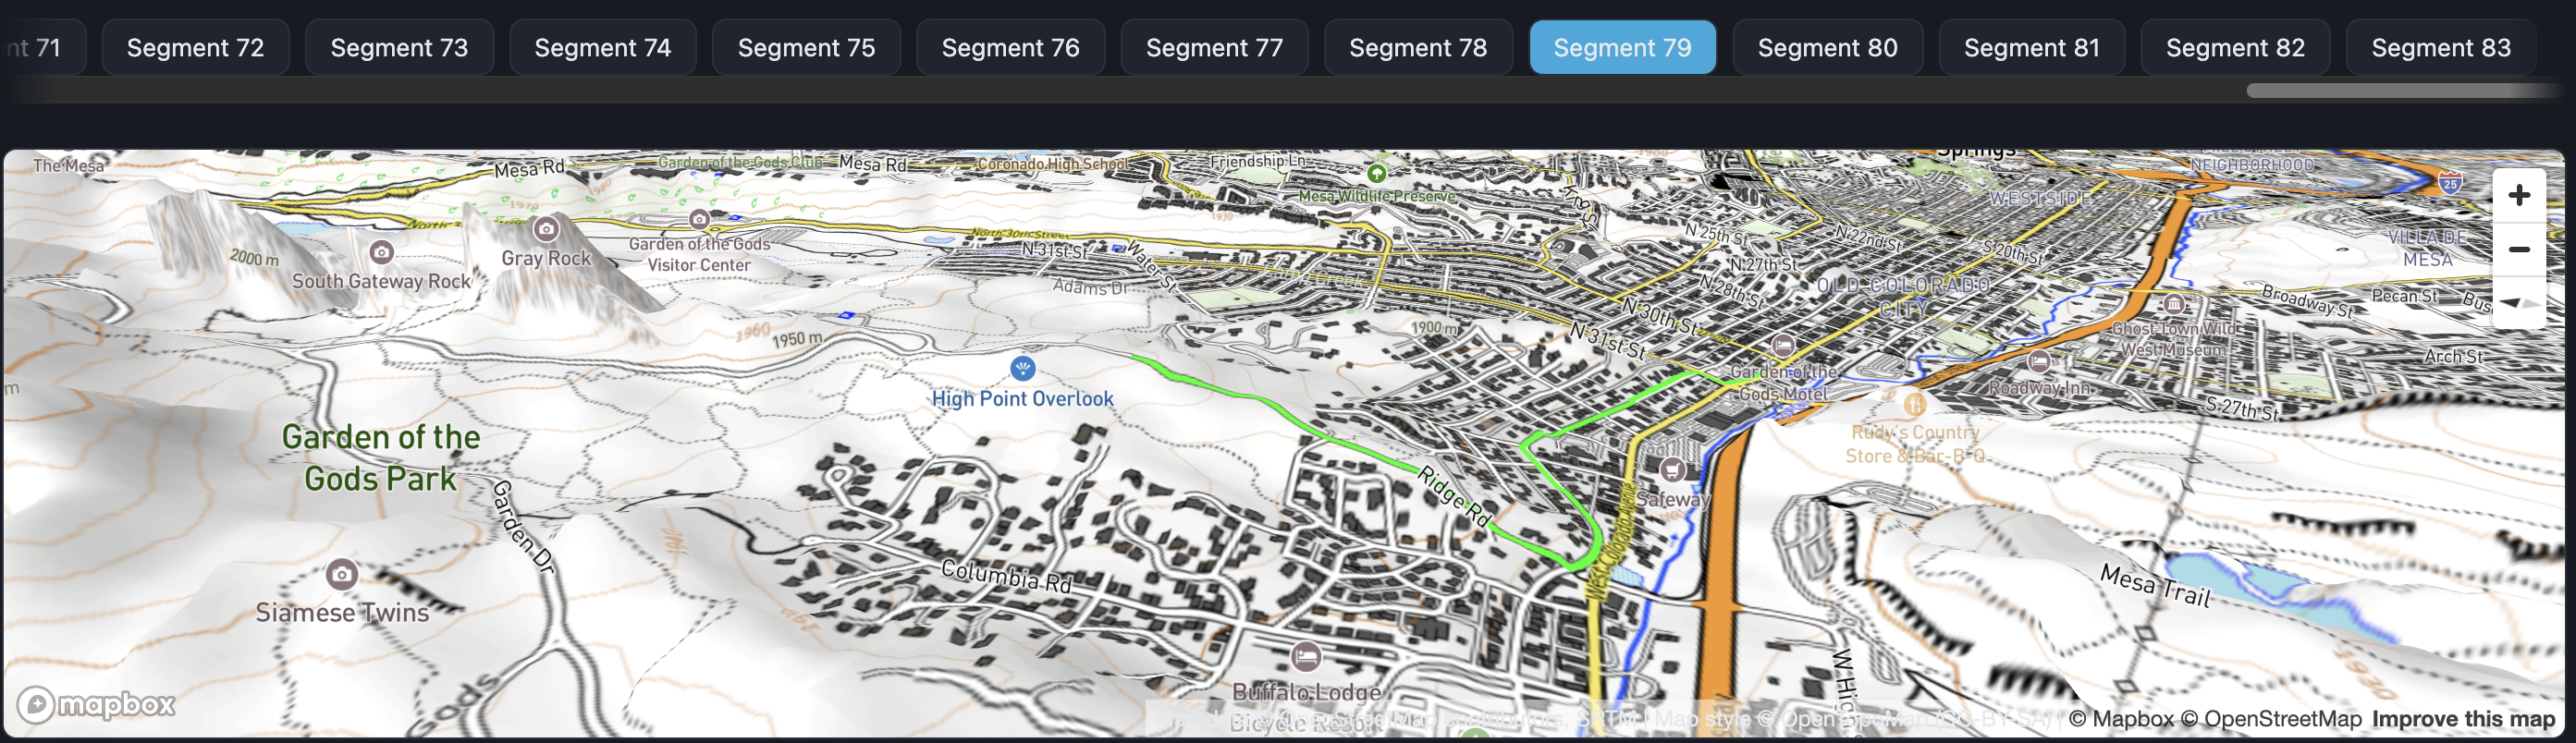
\includegraphics[width=\linewidth]{segment_controls.png}
    \caption{Segmentation options.}
    \label{fig:seg-controls}
  \end{subfigure}
  \caption{Signal plots, wavelet parameters, and segmentation settings.}
  \label{fig:signal-wavelet}
\end{figure}

% === Extensions ===
\section{Extensions Graph}
\label{sec:extensions-compare}
\begin{figure}[H]
  \centering
  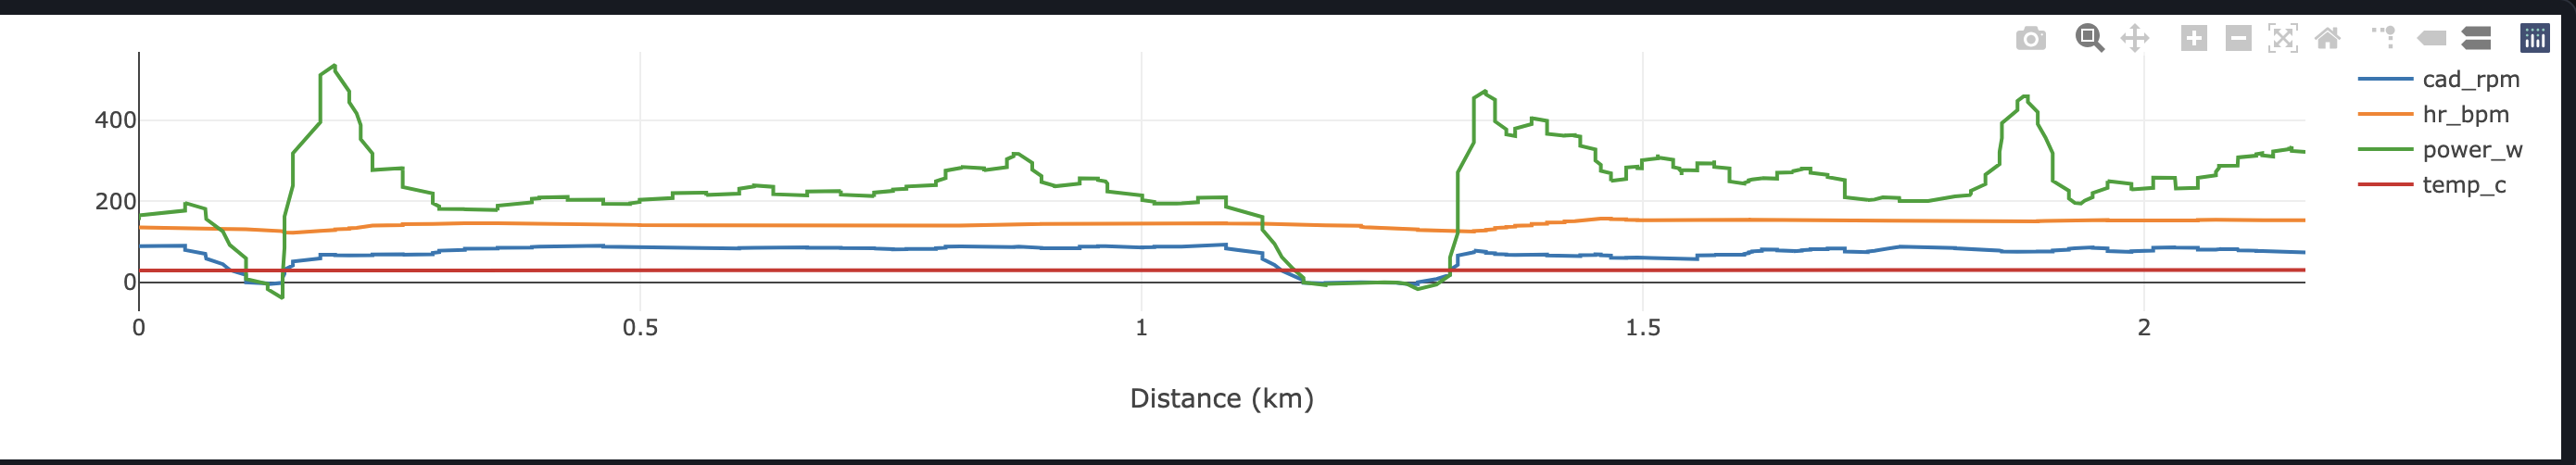
\includegraphics[width=0.7\linewidth]{segment_extensions.png}
  \caption{Auxiliary signals (extensions) aligned to distance.}
  \label{fig:extensions-compare}
\end{figure}

% === External Comparisons ===
\subsection{External Platform Views}
\label{sec:external-views}
\begin{figure}[H]
  \centering
  \begin{subfigure}[b]{0.38\textwidth}
    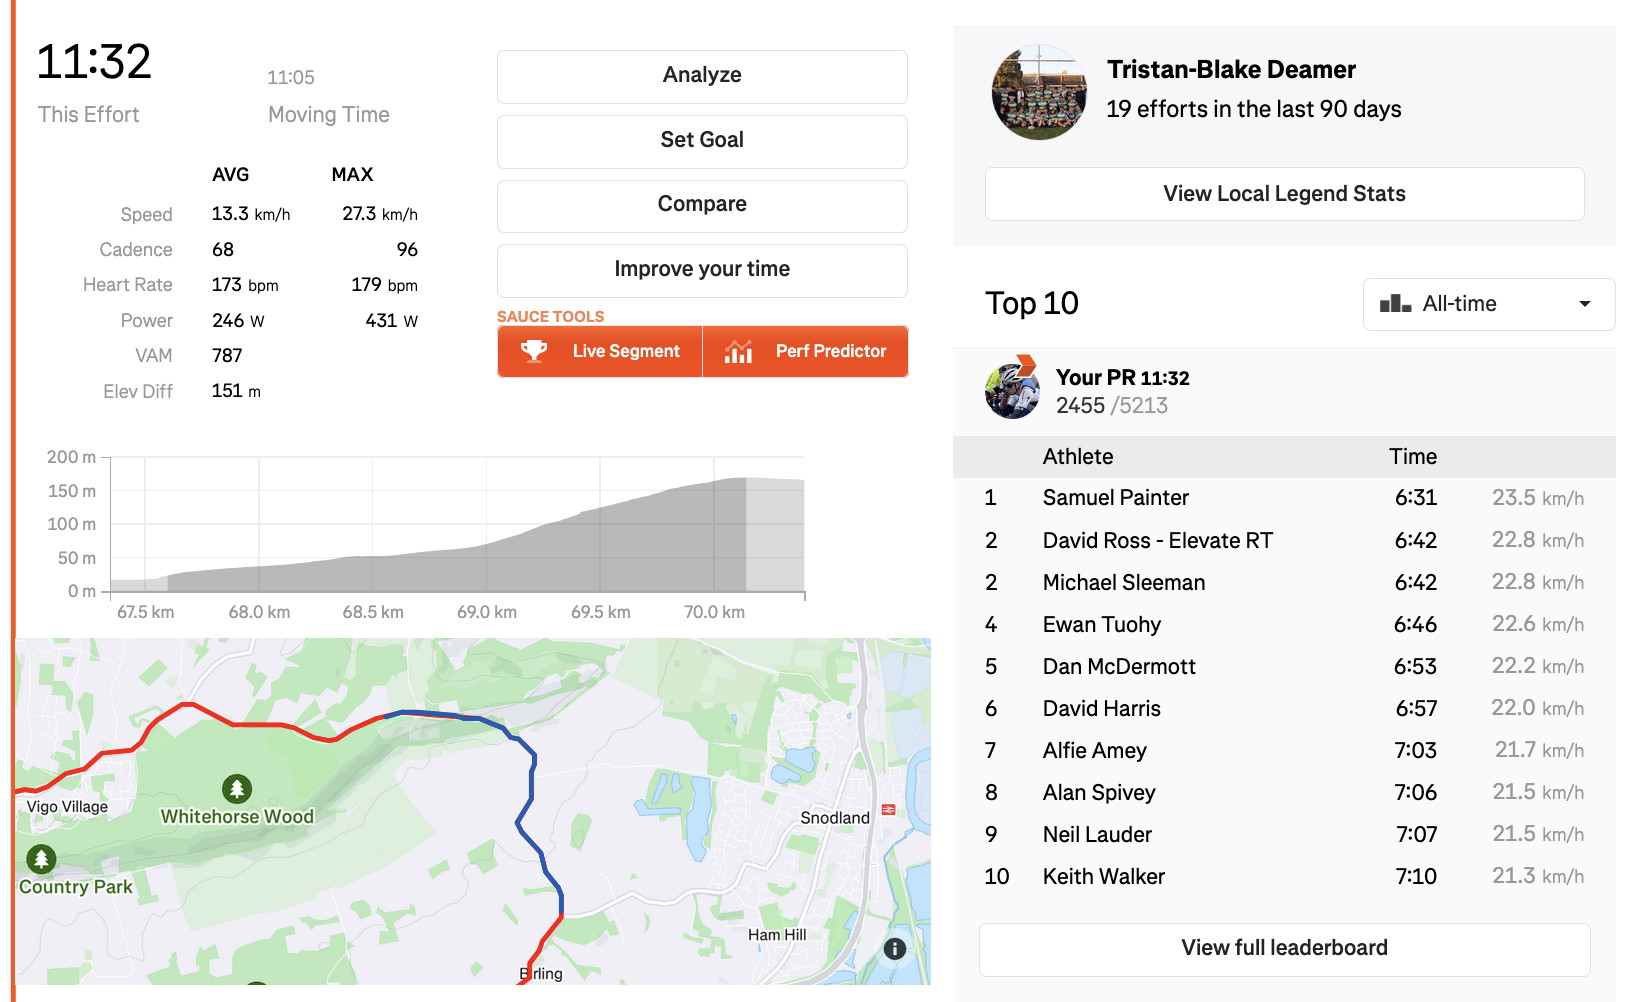
\includegraphics[width=\linewidth]{strava_view.png}
    \caption{Strava route view.}
    \label{fig:strava-view}
  \end{subfigure}\hfill
  \begin{subfigure}[b]{0.38\textwidth}
    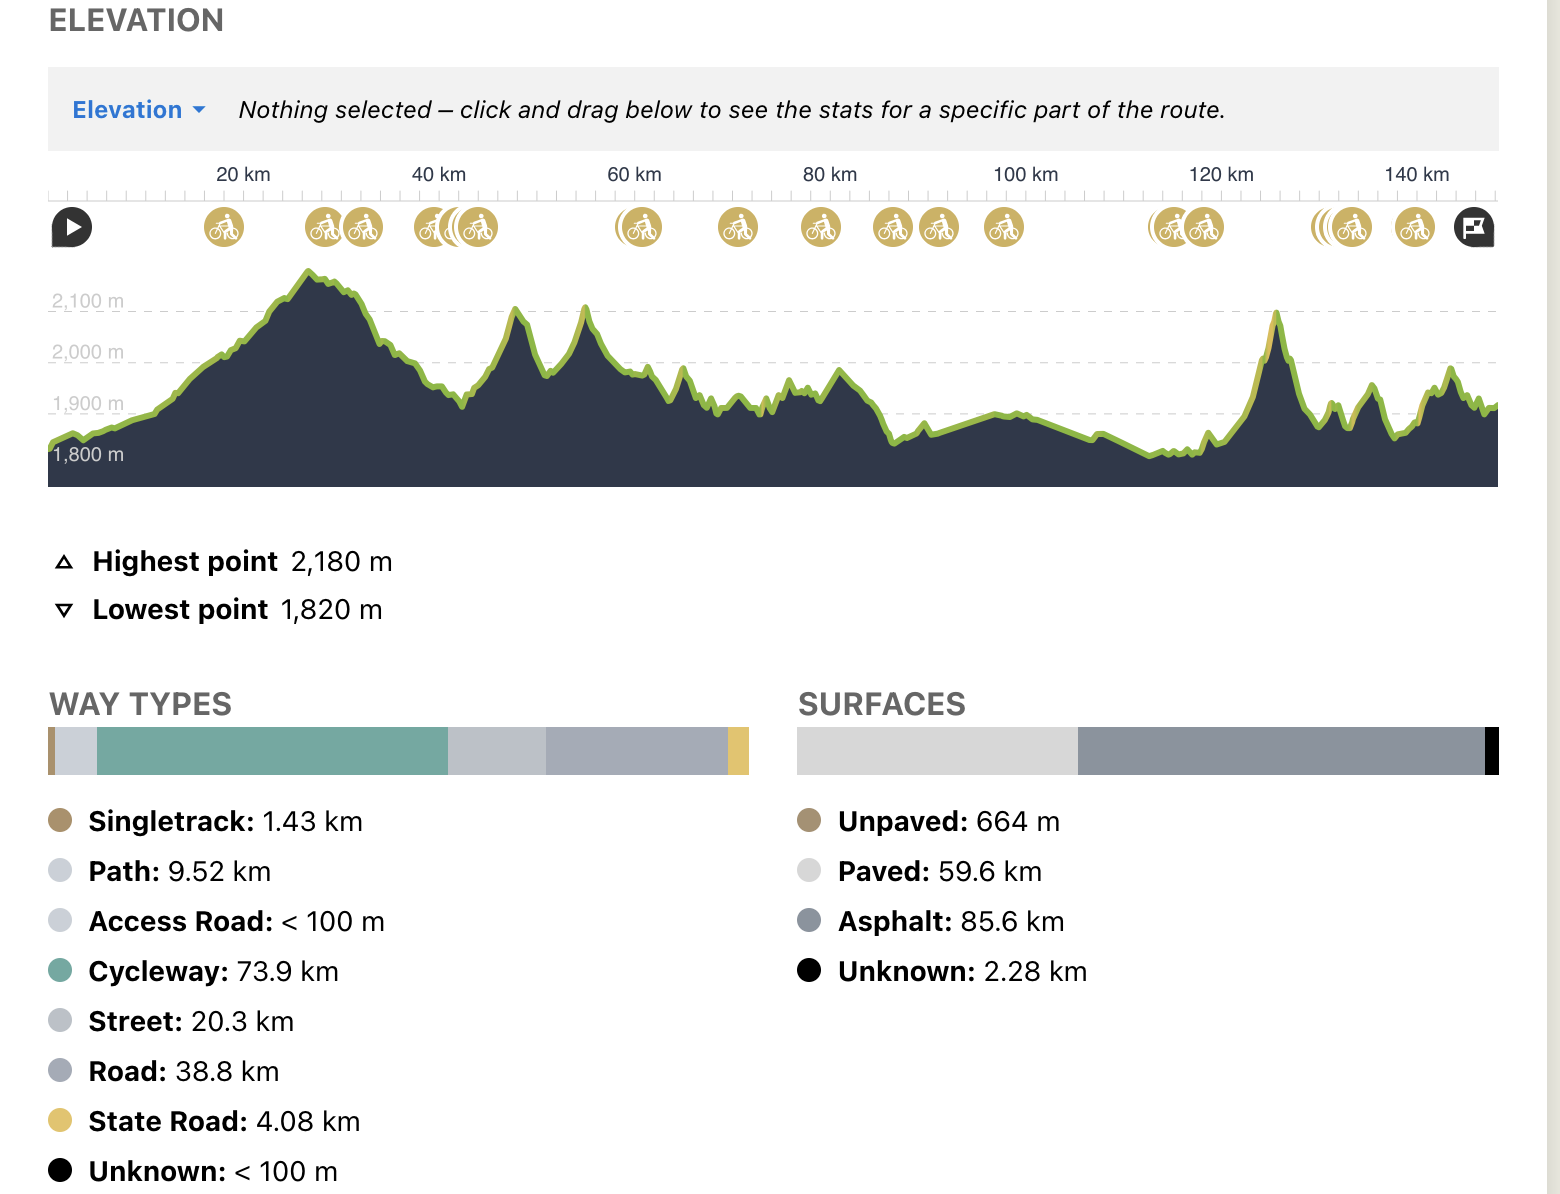
\includegraphics[width=\linewidth]{komoot_view.png}
    \caption{Komoot route view.}
    \label{fig:komoot-view}
  \end{subfigure}
  \caption{Comparison: Strava vs Komoot.}
  \label{fig:external-views}
\end{figure}


\end{document}

